\documentclass[dvipdfmx, a4paper]{jsarticle}
\usepackage[utf8]{inputenc}
\usepackage{graphicx}

\title{総合型選抜入試を意識した技術文書の手引き}
\author{佐藤 雄一}

\begin{document}
\maketitle
\begin{abstract}
この文書は総合型選抜入試の書類作成のために、文書の構成や表や図の書き方について迷わないようガイドになるものを作成しました。技術文書を意識したものになっていますが、文系入試の書類作成の参考になる部分もあるかと思います。

概要には本来は文書全体の概要を書きます。通常の論文では、この先を読むかどうかはここの内容が関心を引くか(自分に必要な内容であるか)で判断される重要な箇所になります。

これから読む人が何が書いてあるかを把握しつつ、興味を引くような書き方を心がけましょう。
\end{abstract}

\section{はじめに}
この文書を本格的に研究や開発に入る前に読み、どんなことを書く必要があるかを把握し、そのために必要な成果物を残すための活動をして、データ等を残しておくと役に立ちます。

もし、この時点で志望校や志望学部が決まっている場合は、入試要項にも必ず目を通して
\begin{itemize}
    \item アドミッションポリシー
    \item 出願資格、条件(資格、履修科目など)
    \item 必要書類
    \item 提出形式(手書きか否か、ファイルフォーマット、枚数など)
\end{itemize}
などの確認をし、不明なことがあれば先方に問い合わせをしましょう。

文書の組み立てとしては基本的にこの文書の章立てに従って(大項目のみ、中項目以下は適当に)おけば問題はないでしょう。逆に、これらが漏れなく書けるように逆算して活動すると良いでしょう。

全体を通じて、時系列に沿って書く必要はないので整理して読みやすく、「自分が書きたいこと」ではなく「読み手が知りたいこと」、アドミッションポリシーとの繋がりが書けているか早い段階から他人にレビューして意見をもらうことが大事です。

\subsection{使用ソフト}
提出先に指定されていなければ、好みの文書作成ソフトを使って構いませんが、見た目も重要な要素なので少ない労力で美しい出力が得られるソフトを選ぶと良いでしょう。

ちなみにこの文書は\LaTeX(レイテック、ラテック、ラテフなどと読みます)というレイアウト(組版)システムを使って書かれています。見た目はシステムに任せて内容を書くことに集中ができ、特に複雑な数式も美しく出力できるため理系の論文によく使われます。

\subsection{見た目}
可能性は低いかもしれませんが白黒印刷されることも考慮して、強調したい場合は色付き文字を使わずに\textbf{太字}などを使い、ページ番号も振りましょう。またハイパーリンクが使える場合も必ずURLを併記しましょう。

\subsection{面接}
面接に関してはデジタルハリウッド大学の「オンライン面接の注意点とマナー、準備すべき10のポイント」\footnote{https://www.dhw.ac.jp/entrance/webinterview/})がオフライン面接についても参考になります。

面接練習は二回は誰かに見てもらいフィードバックをもらうと良いでしょう。

\subsection{資格についての考え方}
場合によれば資格を考慮する試験もあるため資格は持っているに越したことはありませんが、資格には自分の色がついていないということも心得ておく必要があります。

それは、選考をする側から考えると同じ資格を持っているだけの人が複数いた場合は誰を選んでも同じなので競争力がないということを意味します。

そうならないために資格取得を通じた成長を目的として、それを土台に独自の成果を(できれば複数)出しておきましょう。

\section{目的}
この研究や開発の目的を書きます。後の結果と対の内容になるはずです。

始めた動機、きっかけからどうしてこの目的を設定したかを分かりやすく、個性が出るよう具体的なエピソードを交えて書くようにすると良いでしょう。

\section{内容}
研究や開発の内容を記述します。適切にサブセクションに分けると読みやすくなります。

東京工業大学の総合型選抜サイト\footnote{https://admissions.titech.ac.jp/admissions/admission/admission/ao}の「活動実績報告書の例」を見ると、書き方や要求されている水準の参考になります。

後述しますが、結果以降の章の方が重要度が高いとも言えるので開発、研究途中のデータやスクリーンショットは豊富に残し、日誌などを活用して日々の取り組みを記録したりポートフォリオ(作品集)をまとめておきましょう。

共同で取り組んだ場合は、自分が担当した部分とそうでない部分がはっきりわかるように記述しましょう。

また、万が一\footnote{必ずデータは消えると心得ましょう}に備えてバックアップを残しておきましょう。

\subsection{表の書き方}
表題は表番号を付け、表の上部に置きます。表題は長くても構わないので分かりやすい題をつけましょう。左右の罫線は引かない方が技術文書らしくなります。

レイアウトの仕方によっては文と表が離れて配置されることもあるので、文と関係する表は何かを「表の書き方一覧を表\ref{tab:label_how_to_draw_table}に示します。」のように文中に明示します。
 
\begin{table}[htbp]
    \centering
    \caption{表の書き方一覧}
    \label{tab:label_how_to_draw_table}
    \begin{tabular}{c|c} \hline
        タイトル1 & タイトル2 \\ \hline \hline
        アイテム1−1 & アイテム2−1 \\ \hline
        アイテム1−2 & アイテム2−2 \\ \hline
    \end{tabular}
\end{table}

\subsection{図の書き方}
こちらもレイアウトの仕方によっては文と図が離れて配置されることもあるので、文と関係する図は何かを「出力された虎の図を図\ref{fig:label_tiger}に示します。」のように文中に明示します。

図には絵の他にグラフなども含まれます。デジタル化することが難しいものの場合は手書きの図を貼り付け(スキャンや糊付け)ても構いません。

\begin{figure}[htbp]
    \centering
    
\includegraphics[width=4cm, clip]{examples_tiger.eps}
    \caption{虎の画像}
    \label{fig:label_tiger}
\end{figure}

\subsection{実験記録}
実験をする場合は実施した
\begin{itemize}
    \item 年月日
    \item 温度
    \item 湿度
\end{itemize}
や、測定機器については表\ref{tab:label_measure_table}の測定機器の記録例に示した項目を記録しておきましょう。

それぞれの項目の意味は
\begin{description}
    \item[メーカー名] 型番と合わせて製品を特定するため
    \item[型番] 製品を特定するため
    \item[シリアルナンバー] 個体を識別するため
\end{description}
になります。これらは再現実験の際に条件を揃えるためにも必要です。

それぞれを探すために図\ref{fig:tester_front}にメーカー名と型番の例を、図 \ref{fig:tester_back}にシリアルナンバーの例を示します。

\begin{table}[htbp]
    \centering
    \caption{測定機器の記録例}
    \label{tab:label_measure_table}
    \begin{tabular}{c|c|c|c} \hline
        機器名 & メーカー名 & 型番 & シリアルナンバー \\ \hline \hline
        アナログテスタ & CUSTOM & CX-160 MB & 00013310 \\ \hline
        デジタルマルチメータ & CUSTOM & M-02N & P03 \\ \hline
    \end{tabular}
\end{table}

\begin{figure}[htbp]
    \centering
    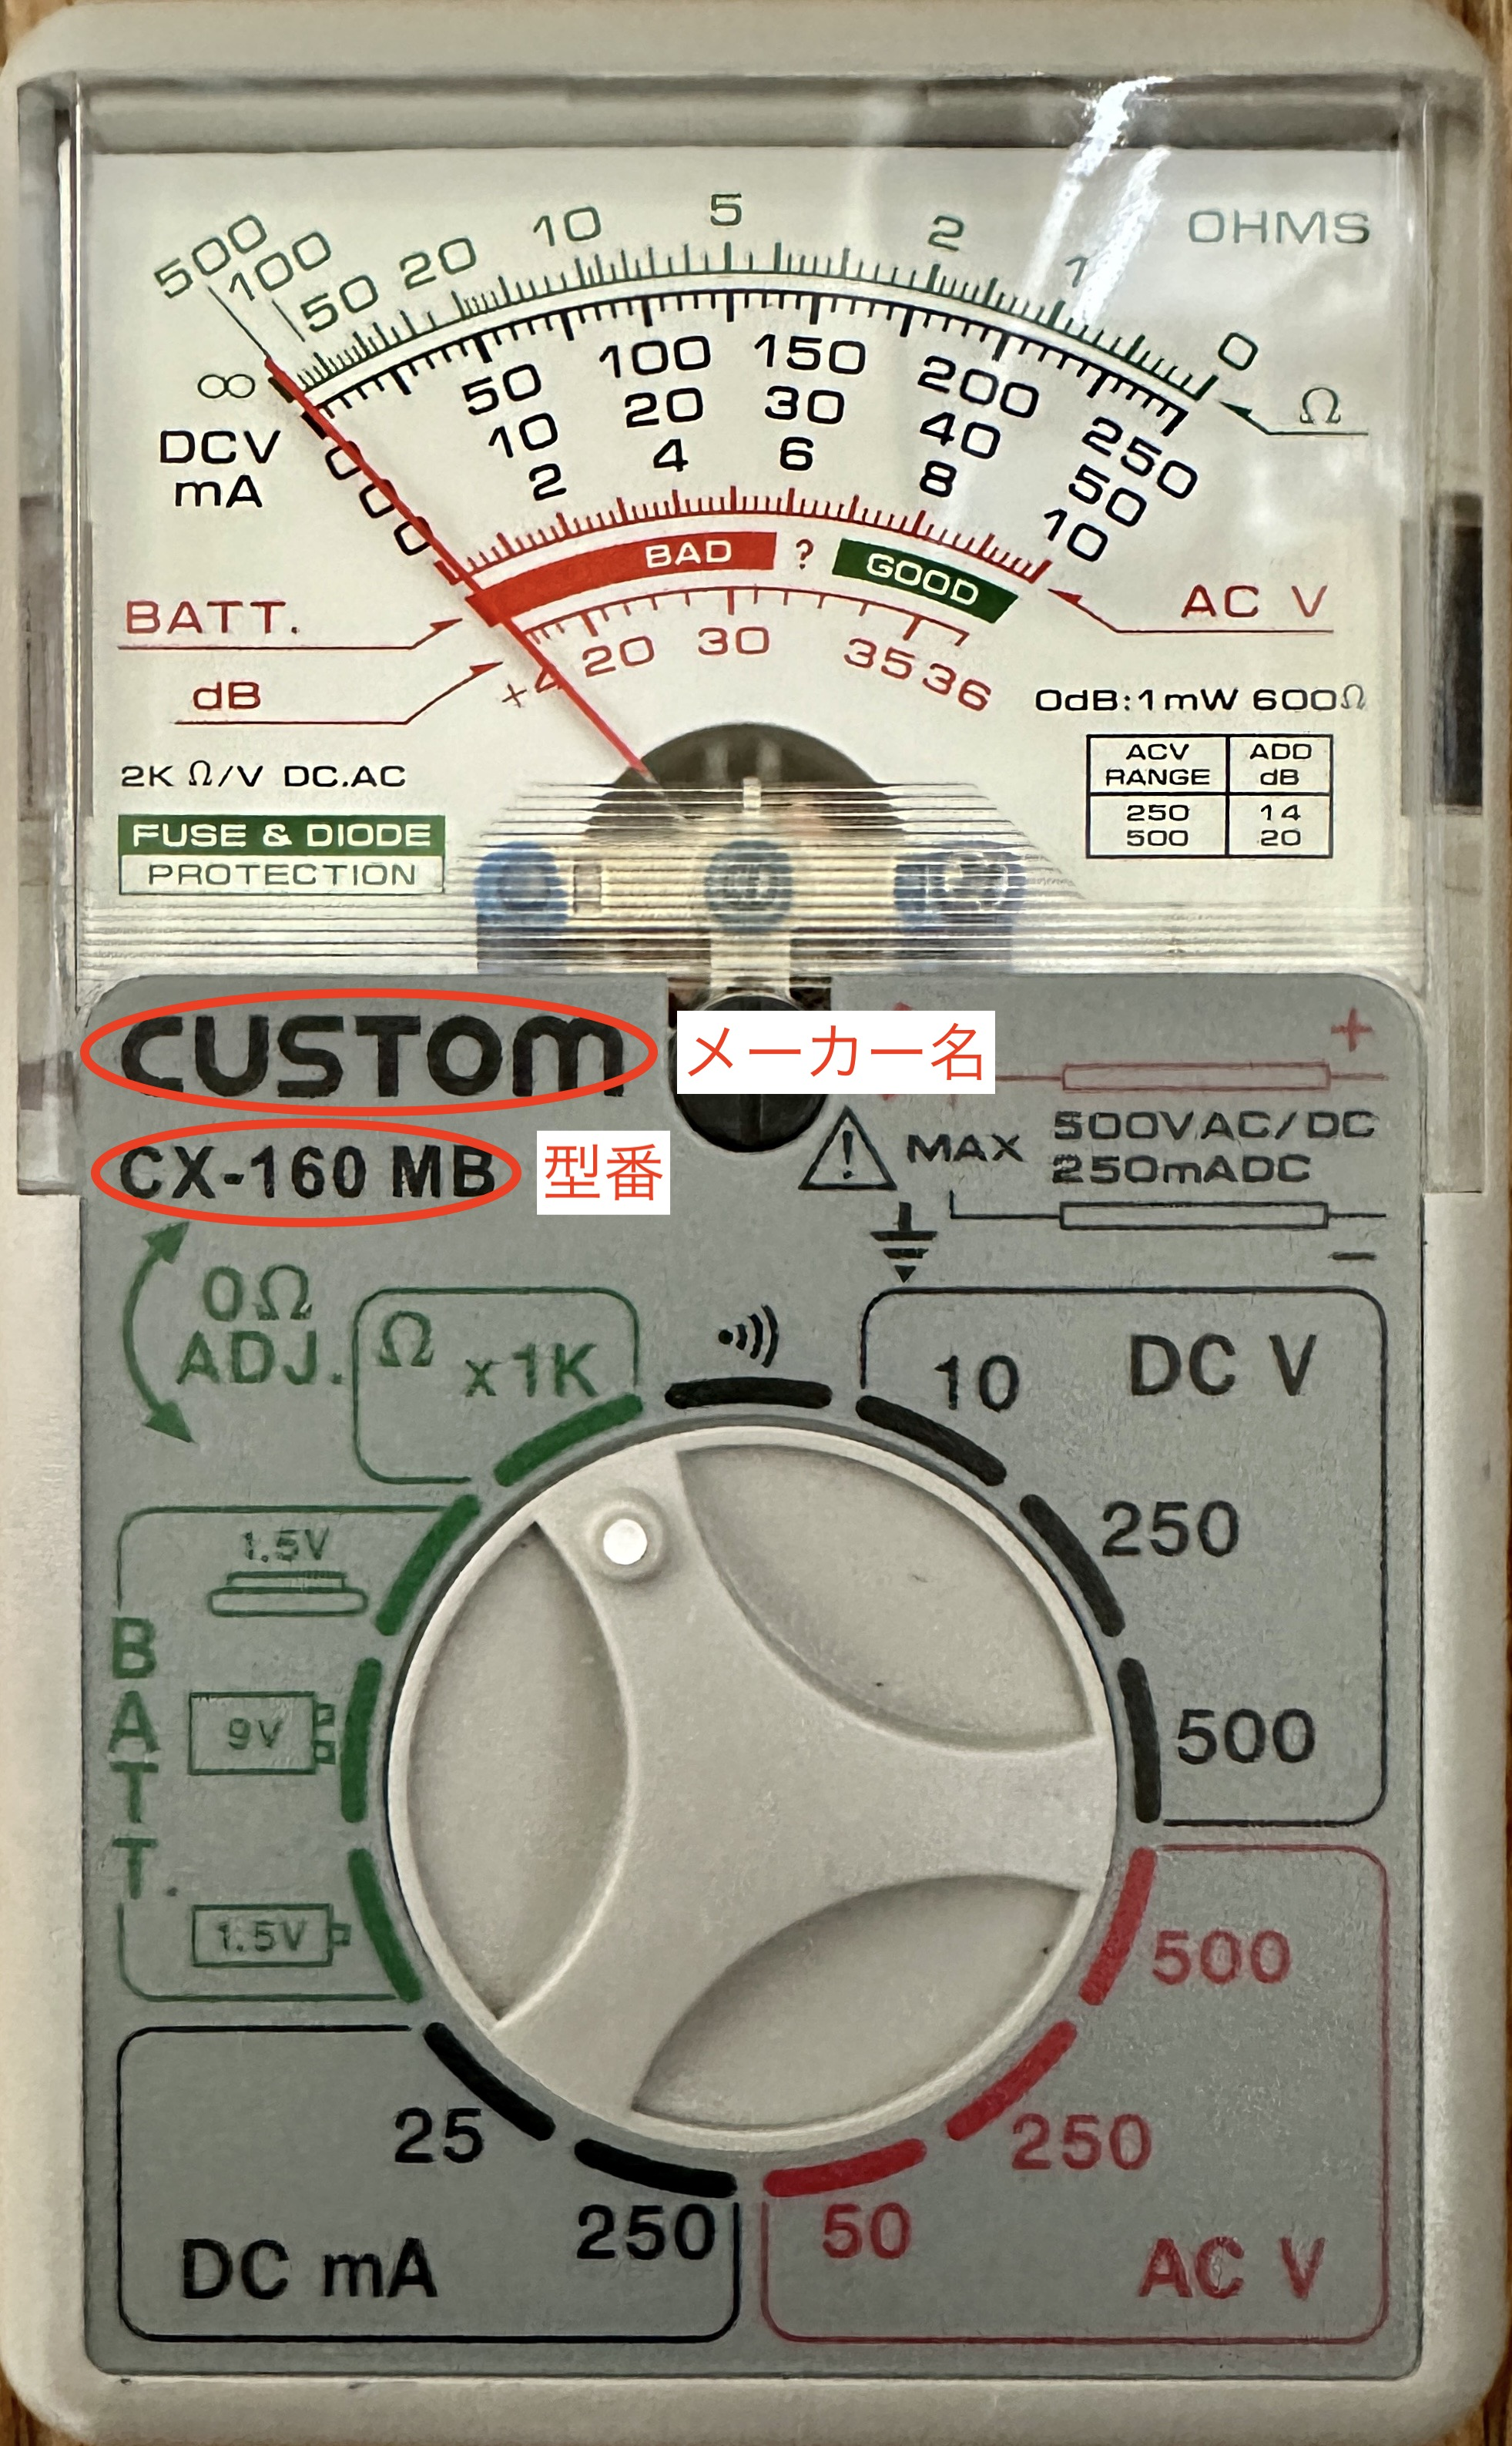
\includegraphics[width=4cm, clip]{tester_front.jpg}
    \caption{メーカー名と型番の例}
    \label{fig:tester_front}

    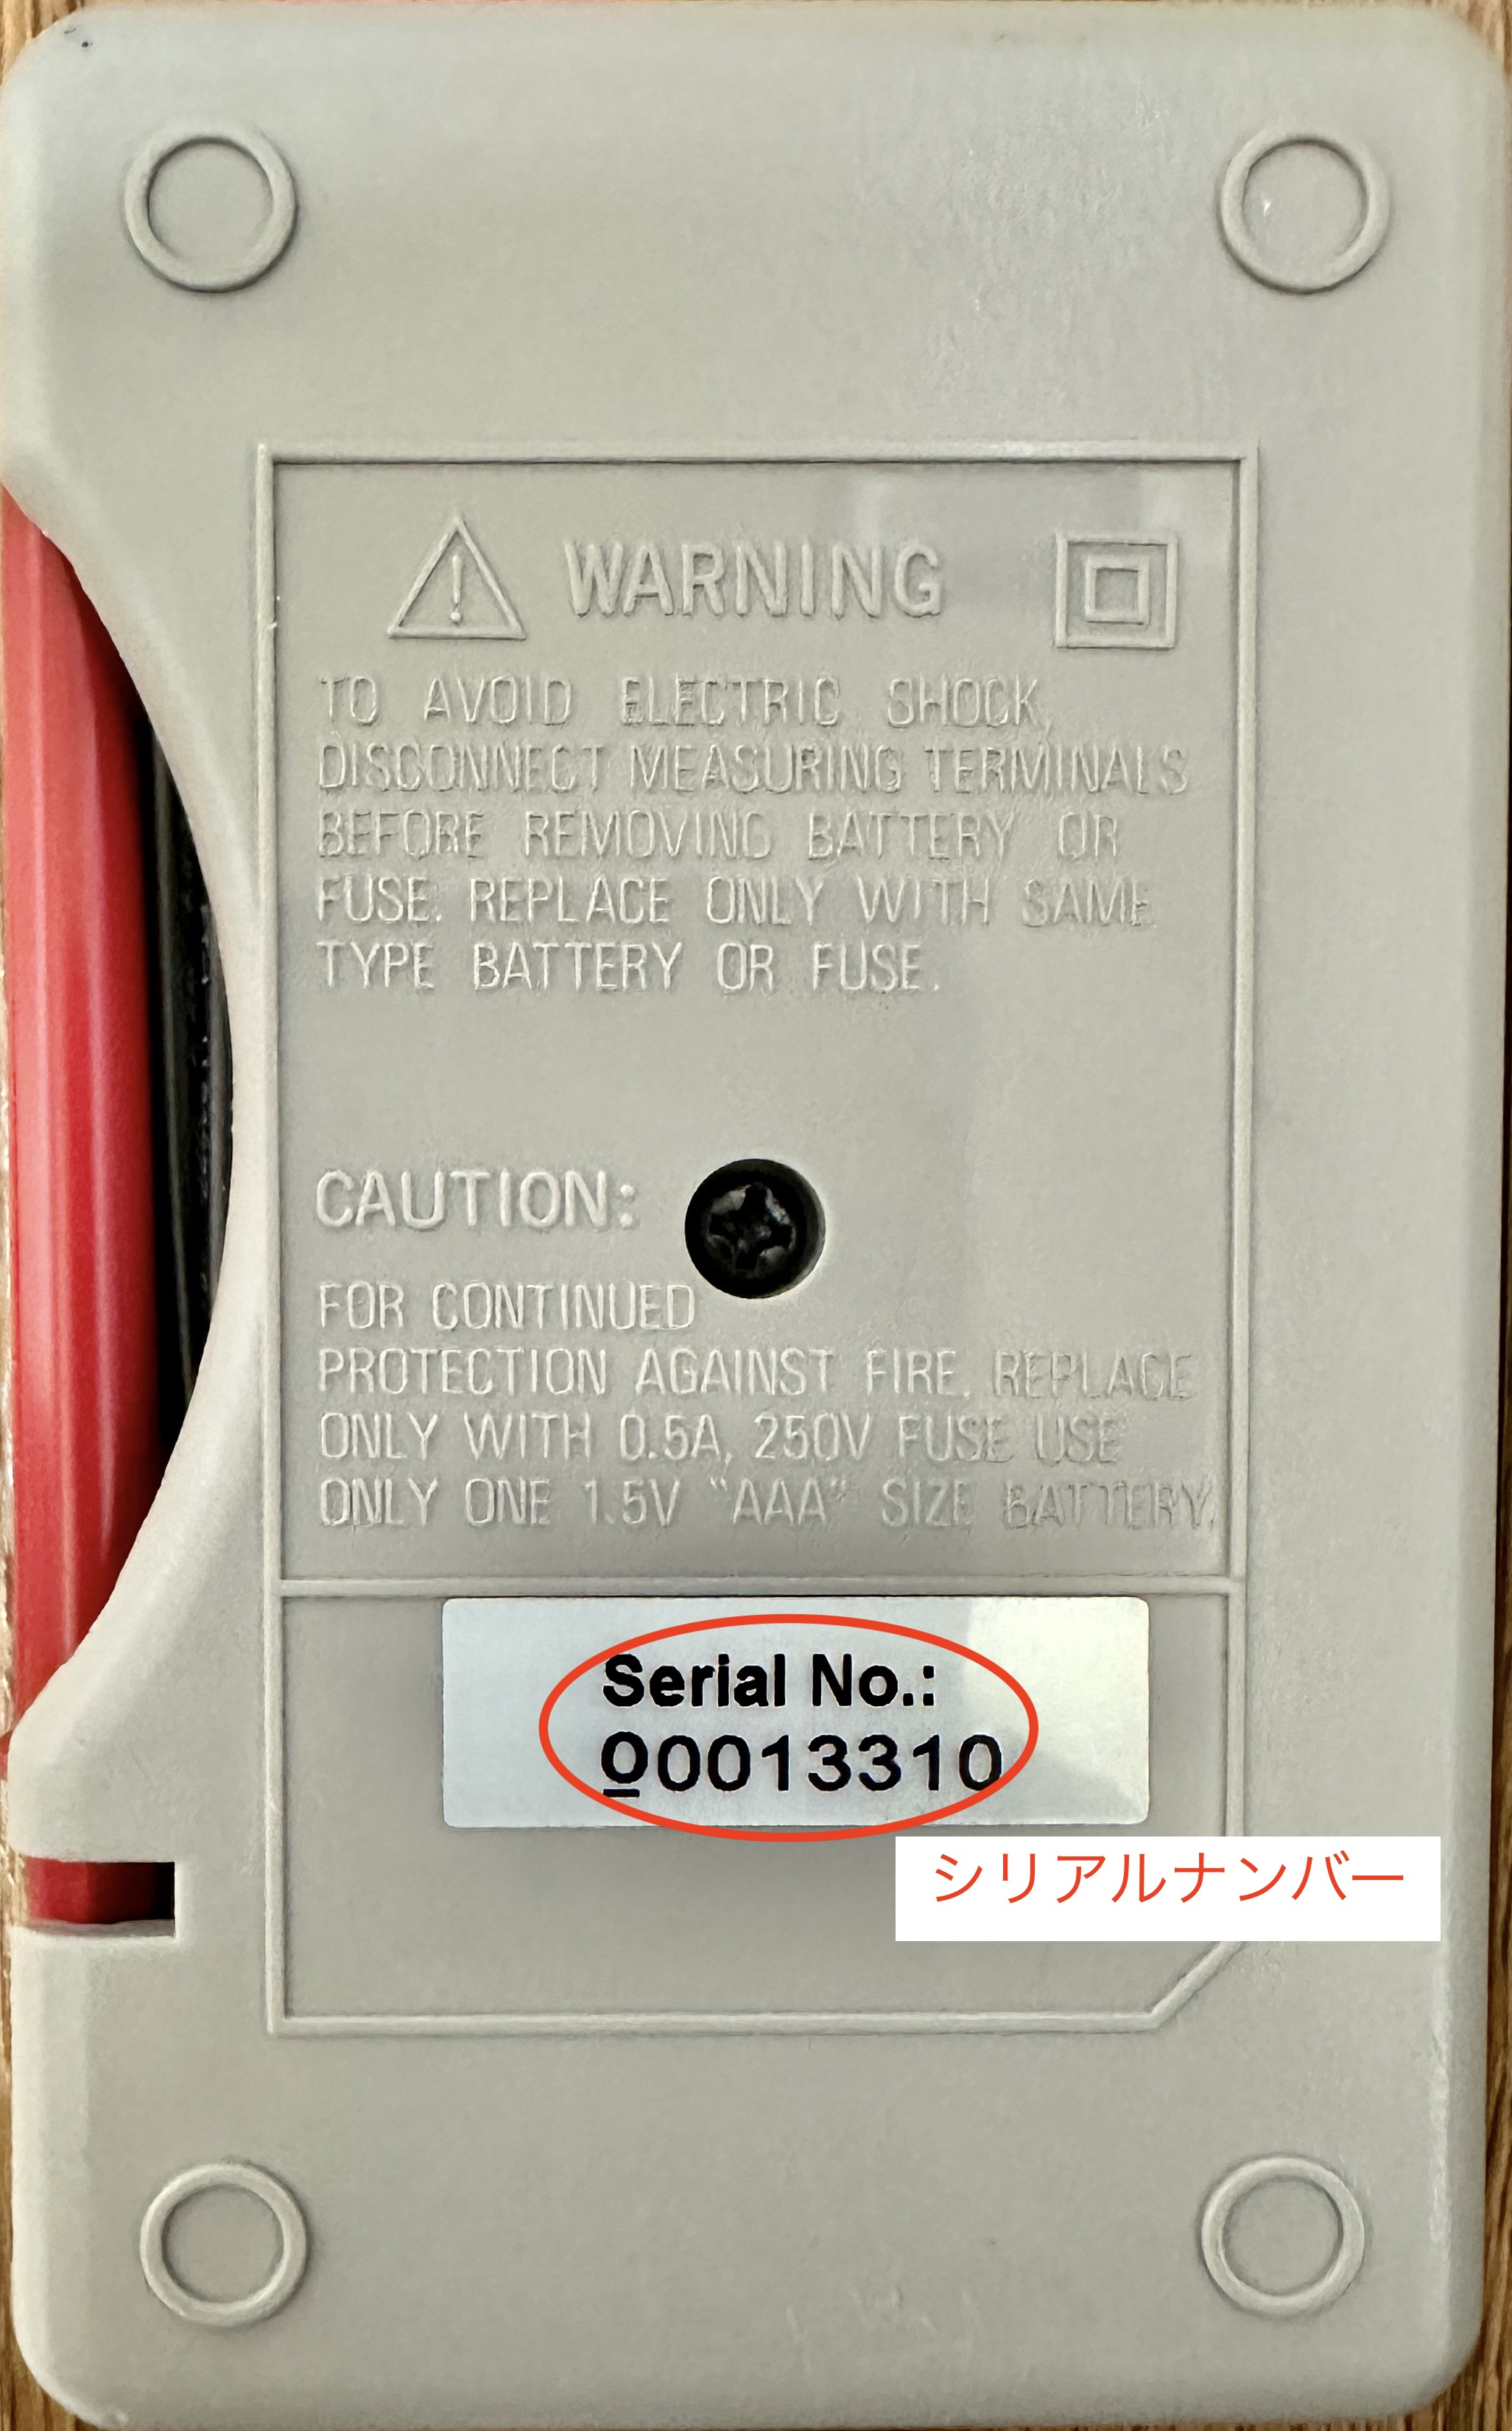
\includegraphics[width=4cm, clip]{tester_back.jpg}
    \caption{シリアルナンバーの例}
    \label{fig:tester_back}
\end{figure}

\subsection{使用したソフトウェア}
使用ソフトウェア(OS/コンパイラ/IDE/ライブラリなど)に関しては
\begin{itemize}
    \item メーカー名
    \item ソフトウェア名
    \item バージョン番号
    \item URL
\end{itemize}

などを記録しておき、どんな開発環境であったかを記述します。開発途中でバージョンが変わった場合は最終的に動作させたバージョンのみで構いません。

\section{結果}
結果を書きます。途中経過を含めて図や表などを用いてわかりやすく記述しましょう。

期待していた結果が出たかどうかは重要でないので、たとえ期待はずれの結果となったとしてもありのままを書くようにしましょう。

そのためにも途中経過をきちんと記録しておくことが大切です。

\section{考察}
ある意味ではこの章以降が内容や結果よりも重要になります。
\begin{itemize}
    \item どんな結果になったか
    \item なぜそのような結果になったか
    \item そこからどのような結論が導かれたか
\end{itemize}
というところにこそ自分らしさが出ると共に、どれくらい一生懸命に取り組んだのかが現れるからです。

\section{今後の展望}
考えられる改良点や応用を書きます。入学後にやりたいことと結びつけて書くのも良いでしょう。

\section{おわりに}
結びの文を書きます。活動を通して自分に起こった変化を書いても面白いと思います。

最後に次のように参考文献を列挙します。参考文献の書き方は書籍やweb記事それぞれで決まっているので調べて、それに従って列挙しましょう。

\subsection{仕上げのポイント}
冗長なところがないかどうかを確認し、これ以上削れない、必要なものだけが残っている状態が理想です。

何においてもそうですが、提出に余裕を持って仕上げるようにしましょう。最終チェックをしていると誤字など直したいところが見つかるものです。そういったところを無くすことが最終的な完成度を上げることに繋がります。

\begin{thebibliography}{9}
\item
奥村晴彦『[改訂第4版] \LaTeXe 美文書作成入門』
(技術評論社, 2007)
\end{thebibliography}

\end{document}
